%----------------------------------------------------------------------------------------
%	SOLUTION 1
%----------------------------------------------------------------------------------------
\subsection*{Problem 1}
\paragraph{1.(a) Proof of $(AB)^T = B^TA^T$:}By definition, if $A \in \mathbb{R}^{m\times n}$ and $B \in \mathbb{R}^{n \times p}$, the $ij$ entry of $AB$,
\begin{align*}
	(AB)_{ij} = \sum_{k=1}^{n}a_{ik}b_{kj},
\end{align*}
where $a_{ik}$ is the $ik$ entry of $A$ and $b_{kj}$ is the $kj$ entry of $B$, $i \in \{1,2,\ldots,m\}, j \in \{1,2,\ldots,p\}$. Now, again by definition of transpose,
\begin{align*}
	(AB)^T_{ij} = (AB)_{ji} = \sum_{k=1}^{n} a_{jk}b_{ki}.
\end{align*}
Now,
\begin{align*}
	(B^TA^T)_{ij} &= \sum_{k=1}^{n}(B^T)_{ik}(A^T)_{kj}\\
	&= \sum_{k=1}^{n} b_{ki}a_{jk}\\
	&= \sum_{k=1}^{n}a_{jk}b_{ki} \\
	&= (AB)^T_{ij}.
\end{align*}
Therefore, $ij$ entry of $(B^TA^T)$ and $(AB)^T$ are equal for all $i \in \{1,2,\ldots,m\}, j \in \{1,2,\ldots,p\}$. Therefore,
\begin{align*}
	(AB)^T = B^TA^T.
\end{align*}
This completes the proof. $\square$
\paragraph{1.(b) Proof of $(AB)^{-1} = B^{-1}A^{-1}$:} Here, it is implied that the inverse of $AB \in \mathbb{R}^{n\times n}, A \in \mathbb{R}^{n \times p}$ and $B \in \mathbb{R}^{p \times n}$ exist. Therefore, let,
\begin{align*}
	&AB = C\\
	\implies& A^{-1}AB = A^{-1}C\\
	\implies& I_{p\times p}B = A^{-1}C\\
	\implies& B = A^{-1}C\\
	\implies& B^{-1}B = B^{-1}A^{-1}C\\
	\implies& I_{n \times n} = B^{-1}A^{-1}C\\
	\implies& I_{n \times n}C^{-1} = B^{-1}A^{-1}CC^{-1}\\
	\implies& C^{-1} = B^{-1}A^{-1}I_{n \times n}\\
	\implies& (AB)^{-1} = B^{-1}A^{-1}.
\end{align*}
This completes the proof. $\square$
\paragraph{1.(c) Proof of $\text{Tr}(AB) = \text{Tr}(BA)$:}By definition, if $A \in \mathbb{R}^{n\times p}$ and $B \in \mathbb{R}^{p \times n}$,
\begin{align*}
	\text{Tr}(AB) &= \sum_{k=1}^{n} (AB)_{kk}\\
	&= \sum_{k=1}^{n} \sum_{j=1}^{p}a_{kj}b_{jk}\\
	&= \sum_{j=1}^{p} \sum_{k=1}^{n}b_{jk}a_{kj}\\
	&= \sum_{j=1}^{p}(BA)_{jj}\\
	&= \text{Tr}(BA).
\end{align*}
This completes the proof. $\square$
%----------------------------------------------------------------------------------------
%	SOLUTION 2
%----------------------------------------------------------------------------------------
\subsection*{Problem 2}
Let, $A \in \mathbb{R}^{n \times p}$ and $B \in \mathbb{R}^{p \times n}$. We have to find $\frac{\partial}{\partial A}\text{Tr}(AB)$. Now,
\begin{align*}
	\frac{\partial}{\partial A} \text{Tr}(AB) &= \frac{\partial}{\partial A} \left[\sum_{k=1}^{n}\sum_{j=1}^{p}a_{kj}b_{jk}\right]\\
	&= \begin{bmatrix}\frac{\partial}{\partial a_{11}} \left[\sum_{k=1}^{n}\sum_{j=1}^{p}a_{kj}b_{jk}\right] & \ldots & \frac{\partial}{\partial a_{1p}} \left[\sum_{k=1}^{n}\sum_{j=1}^{p}a_{kj}b_{jk}\right]\\
	\vdots & \ldots & \vdots\\
	\frac{\partial}{\partial a_{n1}} \left[\sum_{k=1}^{n}\sum_{j=1}^{p}a_{kj}b_{jk}\right] & \ldots & \frac{\partial}{\partial a_{np}} \left[\sum_{k=1}^{n}\sum_{j=1}^{p}a_{kj}b_{jk}\right]\end{bmatrix}\\
	&= \begin{bmatrix}b_{11} & \ldots & b_{p1}\\
	\vdots & \ldots & \vdots\\
	b_{1n} & \ldots & b_{pn}\end{bmatrix}\\
	&= B^T.
\end{align*}
%----------------------------------------------------------------------------------------
%	SOLUTION 3
%----------------------------------------------------------------------------------------
\subsection*{Problem 3}
It is given that,
\begin{align*}
	\begin{bmatrix}A & A\\B & A\end{bmatrix}\begin{bmatrix}A\\C\end{bmatrix} = \begin{bmatrix}0\\I\end{bmatrix}.
\end{align*}
Therefore, by definition of block matrix multiplication,
\begin{align*}
	A^2 + AC &= 0\\
	BA + AC &= I.
\end{align*}
Solving the above two equations for $B$ and $C$, we get,
\begin{align*}
	C &= -A\\
	B &= A^{-1}+A.
\end{align*}
%----------------------------------------------------------------------------------------
%	SOLUTION 4
%----------------------------------------------------------------------------------------
\subsection*{Problem 4}
It is given that,
\begin{align*}
	P = \begin{bmatrix}1 & 2 & 2\\0 & 3 & 1\\0 & 1 & 2\end{bmatrix}.
\end{align*}
Let,
\begin{align*}
	A &= \begin{bmatrix}1 & 0 & 0\\0 & 2 & 0\\0 & 0 & 1\end{bmatrix}\\
	B &= \begin{bmatrix}2\\1\\1\end{bmatrix}\\
	C &= \begin{bmatrix}0 & 1 & 1\end{bmatrix}\\
	D &= 1.
\end{align*}
Therefore, it can be verified that,
\begin{align*}
	A+BD^{-1}C = P.
\end{align*}
Also,
\begin{align*}
	A^{-1} &= \begin{bmatrix}1 & 0 & 0\\0 & \frac{1}{2} & 0\\0 & 0 & 1\end{bmatrix}\\
	CA^{-1} &= \begin{bmatrix}0 & 1 & 1\end{bmatrix}\begin{bmatrix}1 & 0 & 0\\0 & \frac{1}{2} & 0\\0 & 0 & 1\end{bmatrix} = \begin{bmatrix}0 & \frac{1}{2} & 1\end{bmatrix}\\
	D+CA^{-1}B &= 1+\begin{bmatrix}0 & \frac{1}{2} & 1\end{bmatrix}\begin{bmatrix}2\\1\\1\end{bmatrix} = 1+\frac{1}{2}+1 = \frac{5}{2}.
\end{align*}
Therefore, using the matrix inversion lemma,
\begin{align*}
	P^{-1} &= (A+BD^{-1}C)^{-1}\\
	&= A^{-1}-A^{-1}B(D+CA^{-1}B)^{-1}CA^{-1}\\
	&= \begin{bmatrix}1 & 0 & 0\\0 & \frac{1}{2} & 0\\0 & 0 & 1\end{bmatrix}-\begin{bmatrix}1 & 0 & 0\\0 & \frac{1}{2} & 0\\0 & 0 & 1\end{bmatrix}\begin{bmatrix}2\\1\\1\end{bmatrix}\left(\frac{5}{2}\right)^{-1}\begin{bmatrix}0 & \frac{1}{2} & 1\end{bmatrix}\\
	&= \begin{bmatrix}1 & 0 & 0\\0 & \frac{1}{2} & 0\\0 & 0 & 1\end{bmatrix}-\begin{bmatrix}1 & 0 & 0\\0 & \frac{1}{2} & 0\\0 & 0 & 1\end{bmatrix}\begin{bmatrix}2\\1\\1\end{bmatrix}\begin{bmatrix}0 & \frac{1}{5} & \frac{2}{5}\end{bmatrix}\\
	&= \begin{bmatrix}1 & 0 & 0\\0 & \frac{1}{2} & 0\\0 & 0 & 1\end{bmatrix}-\begin{bmatrix}2\\\frac{1}{2}\\1\end{bmatrix}\begin{bmatrix}0 & \frac{1}{5} & \frac{2}{5}\end{bmatrix}\\
	&= \begin{bmatrix}1 & 0 & 0\\0 & \frac{1}{2} & 0\\0 & 0 & 1\end{bmatrix}-\begin{bmatrix}0 & \frac{2}{5} & \frac{4}{5}\\0 & \frac{1}{10} & \frac{1}{5}\\0 & \frac{1}{5} & \frac{2}{5}\end{bmatrix}\\
	&= \begin{bmatrix}1 & -0.4 & -0.8\\0 & 0.4 & -0.2\\0 & -0.2 & 0.6\end{bmatrix}.
\end{align*}
%----------------------------------------------------------------------------------------
%	SOLUTION 5
%----------------------------------------------------------------------------------------
\subsection*{Problem 5}
\paragraph{Data preparation:}I have stored the data in the \textit{dataset.txt} file (included with the submission) where the first column represents \textit{year} and the second column represents steel production in million tons corresponding to the years.
\paragraph{Feature scaling:}I have done feature scaling as we will be dealing with polynomials of order $4$ and the minimum and maximum values of the un-scaled year values will be $1946$ and $1956$ respectively. Therefore, without scaling, the measurement matrix entry values will be huge which might affect the accuracy while taking matrix inverse. The scaling procedure is described below.

I denote the base year as $1946$ and subtract base year from each year values. Therefore, $0$ represents year $1946$, $1$ represents year $1947$ and so on. Let $t \coloneqq t^{\prime}-base\ year$, where $t^{\prime}$ is the original year value.

Now, I have year values ranging from $0$ to $10$ in the dataset. Once I form the measurement matrices, I use \textit{min-max} scaling to have all the features in the range $[0, 1]$. Let $y$ denote the vector of given steel production values.
%------------------Linear---------------------------%
\paragraph{(a) Linear curve fit:}For this the measurement matrix is:
\begin{align*}
	H_{linear} = \begin{bmatrix}1 & t_0\\ \vdots & \vdots\\1 & t_{10}\end{bmatrix}.
\end{align*}
Our goal is to estimate $\beta = [\beta_0\ \beta_1]^T$ such that the error,
\begin{align*}
	e = y - H_{linear}\beta,
\end{align*}
is minimized in least square sense. Fig.~\ref{fig:fit_linear} shows the plot of original data along with the fitted least square curve.
\begin{figure}[h]
	\centering
	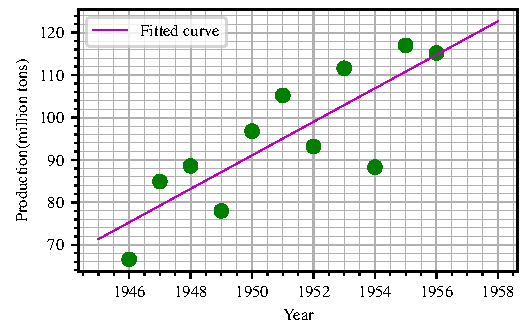
\includegraphics[scale=1.0,trim={0cm 0cm 0cm 0cm},clip]{./code/generatedPlots/fit_linear.pdf}
	\caption{Plot of original data along with fitted linear curve}
	\label{fig:fit_linear}
\end{figure}
%------------------Quadratic---------------------------%
\paragraph{(a) Quadratic curve fit:}For this the measurement matrix is:
\begin{align*}
H_{quadratic} = \begin{bmatrix}1 & t_0 & t_0^2\\ \vdots & \vdots & \vdots\\1 & t_{10} & t_{10}^2\end{bmatrix}.
\end{align*}
Our goal is to estimate $\beta = [\beta_0\ \beta_1\ \beta_2]^T$ such that the error,
\begin{align*}
e = y - H_{quadratic}\beta,
\end{align*}
is minimized in least square sense. Fig.~\ref{fig:fit_quadratic} shows the plot of original data along with the fitted least square curve.
\begin{figure}[h]
	\centering
	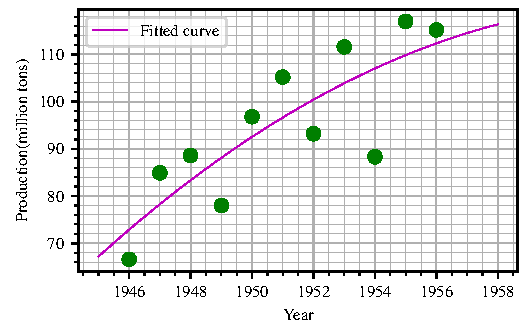
\includegraphics[scale=1.0,trim={0cm 0cm 0cm 0cm},clip]{./code/generatedPlots/fit_quadratic.pdf}
	\caption{Plot of original data along with fitted quadratic curve}
	\label{fig:fit_quadratic}
\end{figure}
%------------------Cubic---------------------------%
\paragraph{(a) Cubic curve fit:}For this the measurement matrix is:
\begin{align*}
H_{cubic} = \begin{bmatrix}1 & t_0 & t_0^2 & t_0^3\\ \vdots & \vdots & \vdots & \vdots\\1 & t_{10} & t_{10}^2 & t_{10}^3\end{bmatrix}.
\end{align*}
Our goal is to estimate $\beta = [\beta_0\ \beta_1\ \beta_2\ \beta_3]^T$ such that the error,
\begin{align*}
e = y - H_{cubic}\beta,
\end{align*}
is minimized in least square sense. Fig.~\ref{fig:fit_cubic} shows the plot of original data along with the fitted least square curve.
\begin{figure}[h]
	\centering
	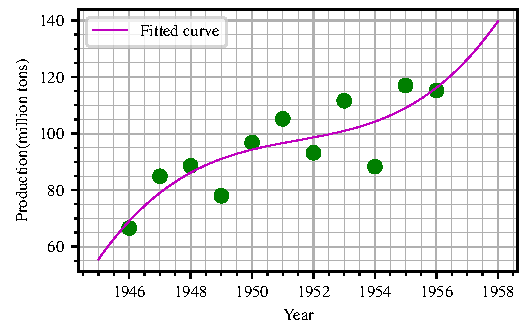
\includegraphics[scale=1.0,trim={0cm 0cm 0cm 0cm},clip]{./code/generatedPlots/fit_cubic.pdf}
	\caption{Plot of original data along with fitted cubic curve}
	\label{fig:fit_cubic}
\end{figure}
%------------------Quartic---------------------------%
\paragraph{(a) Quartic curve fit:}For this the measurement matrix is:
\begin{align*}
H_{quartic} = \begin{bmatrix}1 & t_0 & t_0^2 & t_0^3 & t_0^4\\ \vdots & \vdots & \vdots & \vdots & \vdots\\1 & t_{10} & t_{10}^2 & t_{10}^3 & t_{10}^4\end{bmatrix}.
\end{align*}
Our goal is to estimate $\beta = [\beta_0\ \beta_1\ \beta_2\ \beta_3\ \beta_4]^T$ such that the error,
\begin{align*}
e = y - H_{quartic}\beta,
\end{align*}
is minimized in least square sense. Fig.~\ref{fig:fit_quartic} shows the plot of original data along with the fitted least square curve.
\begin{figure}[h]
	\centering
	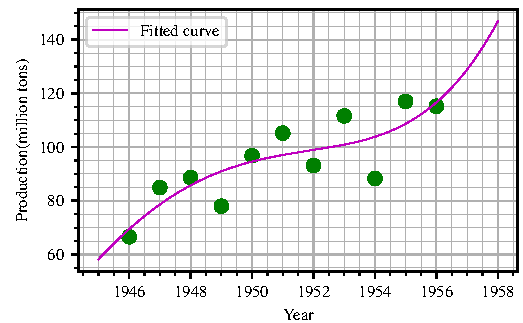
\includegraphics[scale=1.0,trim={0cm 0cm 0cm 0cm},clip]{./code/generatedPlots/fit_quartic.pdf}
	\caption{Plot of original data along with fitted quartic curve}
	\label{fig:fit_quartic}
\end{figure}
\newline
The following table shows the RMS errors and the prediction of steel production in 1957 for each of the polynomial curve fit:
\begin{center}
	\begin{tabular}{||c | c | c ||} 
		\hline
		Polynomial type & RMS error & Prediction of 1957 production (million tons)\\ [0.5ex] 
		\hline\hline
		Linear & $8.782$ & $118.715$\\
		\hline
		Quadratic & $8.666$ & $114.53$\\
		\hline
		Cubic & $8.289$ & $126.188$\\
		\hline
		Quartic & $8.282$ & $128.86$\\ [1ex]
		\hline
	\end{tabular}
\end{center}
 